% ========================================================
% IMPLEMENTACIÓN EN GO
% ========================================================
\section{Implementación en Go}\label{sec:go}

Todo el código vive en el módulo \texttt{tp/kmeans/} del repositorio, escrito con la biblioteca
estándar de Go \cifra{go} y sin dependencias de terceros. La Tabla~\ref{tab:paquete} resume su
estructura.

\begin{table}[H]
\caption{Estructura del paquete \texttt{tp/kmeans}}\label{tab:paquete}
\small
\begin{tabularx}{\textwidth}{@{}L{4.3cm}Y@{}}
\toprule
\textbf{Archivo} & \textbf{Responsabilidad} \\
\midrule
\texttt{gold.go} & Lee el CSV de gold a un arreglo plano de $N \times 6$ \texttt{float64}; rechaza
  \texttt{NaN} e infinitos \\
\texttt{inicializacion.go} & k-means++ con semilla fija; guarda y lee los centroides iniciales con
  su sha256 \\
\texttt{secuencial.go} & Contrato numérico (\texttt{Opciones}, \texttt{Resultado}) y Lloyd en un
  solo hilo \\
\texttt{concurrente.go} & Lloyd con worker pool persistente, bloques por canal y reducción en orden
  (Sección~\ref{sec:sync}) \\
\texttt{estadistica.go} & Media recortada, mediana, desviación e intervalo bootstrap del cociente
  de medias \\
\texttt{metadatos.go}, \texttt{recursos.go} & Máquina, versión de Go, commit, \texttt{GOMAXPROCS};
  memoria y CPU del proceso \\
\texttt{submuestra.go} & Muestreo sistemático reproducible, para el barrido por tamaño \\
\texttt{cmd/kmeans} & CLI que corre una configuración y reporta tiempos, memoria e inercia \\
\texttt{cmd/benchmark} & Protocolo de medición fijado en código (Sección~\ref{sec:speedup}) \\
\bottomrule
\end{tabularx}
\end{table}

\subsection{Versión secuencial}

\texttt{Secuencial} corre Lloyd en un solo hilo con el contrato de la Sección~\ref{sec:promela}. Es
el $T_{\text{secuencial}}$ del speedup, y por eso importa que sea el mismo algoritmo bien escrito y
no una versión degradada: usa el mismo arreglo plano, la misma función de distancia y los mismos
acumuladores por cluster que la versión concurrente. La única diferencia es que recorre los $N$
viajes en un solo bucle. No modifica ni los datos ni los centroides iniciales que recibe.

\subsection{Versión concurrente}

\texttt{Concurrente} recibe las mismas entradas más dos parámetros, \texttt{Workers} y
\texttt{Chunk}, independientes a propósito porque el reparto afecta al rendimiento tanto como la
cantidad de goroutines \parencite{kwedlo2021}. Su funcionamiento se explica en la
Sección~\ref{sec:sync}.

\subsection{Evidencia de funcionamiento}

Las Figuras~\ref{fig:cli-seq} y~\ref{fig:cli-conc} son la salida de la CLI sobre el dataset
completo en la laptop del equipo, con $k = \cifra{k}$ y \cifra{iter-fijas} iteraciones. Los textos
de origen están en \texttt{tp/informe/pc2/img/} junto a las imágenes, y cualquiera puede rehacerlas
con los comandos que encabezan cada captura. Ambas corridas parten del mismo archivo de centroides
iniciales (la primera lo genera y la segunda lo lee, como muestra el \texttt{init 0 ms}), y ambas
terminan con la misma inercia, lo que es la primera comprobación de que calculan lo mismo.

\begin{figure}[H]
\caption{CLI en modo secuencial sobre el dataset completo}\label{fig:cli-seq}
\centering
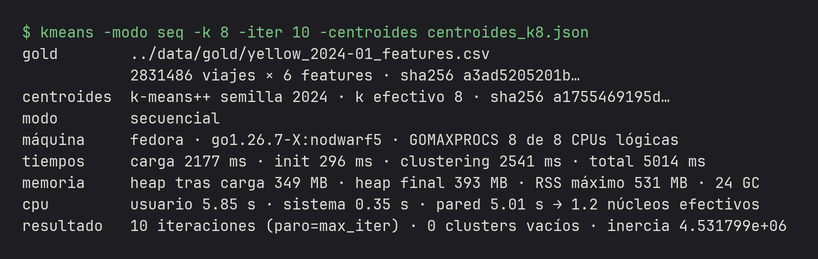
\includegraphics[width=\textwidth]{img/cli-secuencial.png}
\end{figure}

\begin{figure}[H]
\caption{CLI en modo concurrente con 8 workers, mismos centroides iniciales}\label{fig:cli-conc}
\centering
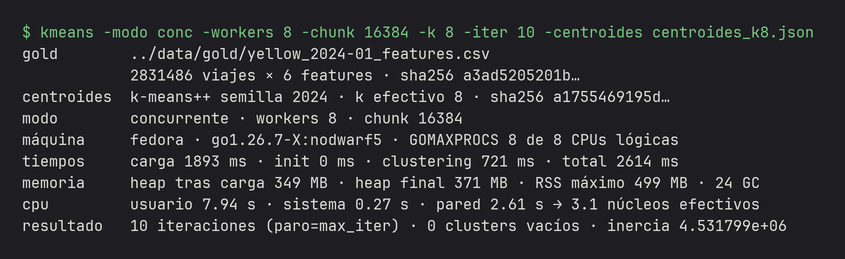
\includegraphics[width=\textwidth]{img/cli-concurrente.png}
\end{figure}

Cada corrida imprime, además del resultado, lo que hace falta para reproducirla: sha256 del gold y
de los centroides iniciales, semilla, máquina, versión de Go y \texttt{GOMAXPROCS}, y los tiempos
separados de carga, inicialización y clustering. Esa separación es la que permite medir el speedup
solo sobre el clustering, que es la parte que la concurrencia puede acelerar.

\subsection{Pruebas y equivalencia entre versiones}\label{sec:equivalencia}

El paquete se escribió con pruebas primero, y todas corren con \texttt{go test -race}, el detector
de carreras de Go, en cada \emph{pull request} mediante GitHub Actions. Un test que pasa sin
\texttt{-race} no demuestra nada sobre una sección crítica. Las pruebas que sostienen la
equivalencia entre versiones son:

\begin{itemize}
  \item con un solo bloque y un solo worker, la versión concurrente es idéntica bit a bit a la
        secuencial (mismo orden de suma);
  \item con $P \in \{1, 2, 3, 4, 8\}$ y bloques pequeños, la versión concurrente da exactamente el
        mismo resultado para todo $P$;
  \item contra la secuencial, con varios bloques, los centroides y la inercia coinciden dentro de una
        tolerancia relativa explícita y las \emph{asignaciones} son las mismas: una inercia parecida
        no demuestra la misma partición, así que se comparan también las etiquetas;
  \item cada punto queda asignado exactamente una vez, con más workers que puntos, con un bloque
        mayor que $N$, con $k = 1$ y con $k = N$;
  \item ninguna versión modifica sus entradas, y ambas informan el mismo motivo de parada.
\end{itemize}

Sobre el gold real, una prueba adicional (que se omite con \texttt{-short}) corre ambas versiones y
comprueba la equivalencia con \cifra{n}~viajes. La Tabla~\ref{tab:inercias} de la
Sección~\ref{sec:reproducibilidad} muestra el resultado de esa comparación en las corridas oficiales.
